% !TEX program = xelatex
% DriveCompose 中文对照稿；会议年份统一为 CVPR 2027。
\documentclass[10pt,twocolumn,letterpaper]{article}
\usepackage[review]{cvpr}
%% This file contains a number of tweaks that are typically applied to the main document.
%% They are not enabled by default, but can be enabled by uncommenting the relevant lines.


%% Standard CVPR float handling is used for the teaser and experiment figures.
\usepackage{placeins} %< keep references after all experiment floats

%%
%% caption and (global) spacing overrides
%%
\usepackage{caption} %< for "\captionof" commands (teaser)
% \setlength{\abovecaptionskip}{.5em} % space above caption
% \setlength{\belowcaptionskip}{1em} % space below caption

%%
%% Inline annotations; for predefined colors, refer to "dvipsnames" in the xcolor package:
%% https://tinyurl.com/overleaf-colors
%%
\newcommand{\red}[1]{{\color{red}#1}}
\newcommand{\todo}[1]{{\color{red}#1}}
\newcommand{\TODO}[1]{\textbf{\color{red}[TODO: #1]}}
%%
%% Disable for camera ready / submission by uncommenting these lines:
%%
% \renewcommand{\TODO}[1]{}
% \renewcommand{\todo}[1]{#1}

%%
%% Work harder in optimizing text layout. Typically shrinks text by 1/6 of page, enable
%% it at the very end of the writing process, when you are just above the page limit.
%%
% \usepackage{microtype}

%%
%% Fine-tune paragraph spacing.
%%
% \renewcommand{\paragraph}[1]{\vspace{.5em}\noindent\textbf{#1.}}

%%
%% Globally adjusts space between figure and caption.
%%
% \setlength{\abovecaptionskip}{.5em}

%%
%% Allows "the use of \paper to refer to the project name"
%% with automatic management of space at the end of the word.
%%
% \usepackage{xspace}
% \newcommand{\paper}{ProjectName\xspace}

%%
%% Commonly used math definitions.
%%
% \DeclareMathOperator*{\argmin}{arg\,min}
% \DeclareMathOperator*{\argmax}{arg\,max}

%%
%% Tighten underline.
%%
% \usepackage{soul}
% \setuldepth{foobar}

%%
%% Reconfigure paragraph (tweaks spacing)
%%






% Portable Times-compatible Unicode fonts; CVPR geometry is unchanged.
\usepackage{iftex}
\ifXeTeX
  \usepackage{fontspec}
  \setmainfont{texgyretermes-regular.otf}[
    BoldFont=texgyretermes-bold.otf,ItalicFont=texgyretermes-italic.otf,
    BoldItalicFont=texgyretermes-bolditalic.otf]
  \setsansfont{texgyreheros-regular.otf}[
    BoldFont=texgyreheros-bold.otf,ItalicFont=texgyreheros-italic.otf,
    BoldItalicFont=texgyreheros-bolditalic.otf]
  \setmonofont{texgyrecursor-regular.otf}[
    BoldFont=texgyrecursor-bold.otf,ItalicFont=texgyrecursor-italic.otf,
    BoldItalicFont=texgyrecursor-bolditalic.otf]
\fi

\usepackage{tikz}
\usepackage{needspace}
\usetikzlibrary{arrows.meta,patterns}
\usepackage{iftex}
\ifXeTeX
  \usepackage{fontspec}
  \usepackage{xeCJK}
  \setCJKmainfont{FandolSong-Regular.otf}[BoldFont=FandolSong-Bold.otf,ItalicFont=FandolKai-Regular.otf]
  \setCJKsansfont{FandolHei-Regular.otf}[BoldFont=FandolHei-Bold.otf]
  \setCJKmonofont{FandolFang-Regular.otf}
\else
  \PackageError{DriveCompose}{The Chinese counterpart requires XeLaTeX}{Compile main_zh.tex with XeLaTeX or Tectonic.}
\fi
\definecolor{cvprblue}{rgb}{0.21,0.49,0.74}
\usepackage[pagebackref,breaklinks,colorlinks,allcolors=cvprblue]{hyperref}
\usepackage{url}
\def\paperID{*****}
\def\confName{CVPR}
\def\confYear{2027}
\title{DriveCompose：面向可组合高斯驾驶世界的观测锚定联合补全}
\author{Anonymous CVPR Submission}
\begin{document}
\maketitle
\begin{abstract}
驾驶日志只覆盖场景的一部分，仿真中的新相机位姿和资产状态却会暴露未见表面。补全这些表面时，需要协调世界空间中的背景、规范空间中的车辆与关节人体，并保持日志记录的外观。我们提出 DriveCompose，通过联合补全分类规范查询，构建可组合的高斯驾驶世界。共享恢复前端提供几何、身份和状态证据；局部查询组保留各类内容的空间结构，全局记忆在背景与资产之间交换上下文。条件流填充未知潜码，每步恢复已见潜码，并抑制已知自由空间。固定的逐查询解码器保持已见高斯参数，独立的渲染检查则识别新增内容造成的退化。候选通过检查后，背景与规范资产保持固定，由相机位姿、刚体变换和骨架姿态驱动不同轨迹的渲染，各条轨迹共享同一次补全结果。该方法将生成过程放在离线世界构建阶段，并通过状态驱动装配明确表达后续场景变化。
\end{abstract}

\begin{figure*}[t]
  \centering
  % Native vector overview; physical canvas 495 x 225 pt at CVPR text width.
% All scene marks are schematic. No experiment results are drawn here.
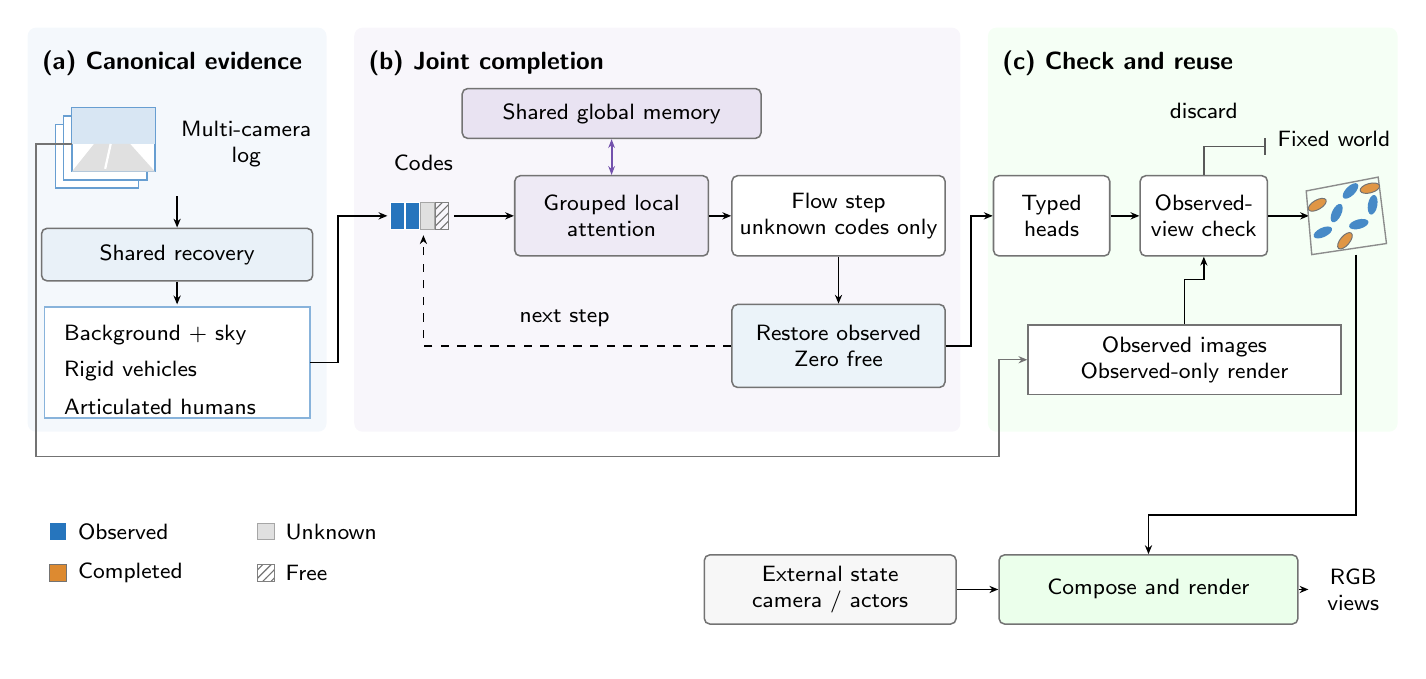
\begin{tikzpicture}[x=1pt,y=1pt,
  every node/.style={font=\sffamily\fontsize{8.3}{9.5}\selectfont,inner sep=2pt,align=center},
  op/.style={draw=black!55,rounded corners=2pt,fill=white,line width=.55pt},
  route/.style={-{Stealth[length=3.2pt,width=2.6pt]},line width=.65pt},
  paneltitle/.style={anchor=west,font=\sffamily\bfseries\fontsize{9.5}{11}\selectfont,inner sep=0pt}]
\path[use as bounding box] (0,0) rectangle (495,225);
\definecolor{dcobs}{HTML}{2675BD}
\definecolor{dcnew}{HTML}{DD8A30}
\definecolor{dcmem}{HTML}{7351AD}
\fill[dcobs!5,rounded corners=3pt] (0,79) rectangle (108,225);
\fill[dcmem!5,rounded corners=3pt] (118,79) rectangle (337,225);
\fill[green!4,rounded corners=3pt] (347,79) rectangle (495,225);
\node[paneltitle] at (5,212) {(a) Canonical evidence};
\node[paneltitle] at (123,212) {(b) Joint completion};
\node[paneltitle] at (352,212) {(c) Check and reuse};

% Camera observations: stacked image planes, kept distinct from query tensors.
\foreach \dx/\dy in {0/0,3/3,6/6}{
  \draw[fill=white,draw=dcobs!70,line width=.6pt] (10+\dx,167+\dy) rectangle (40+\dx,190+\dy);
}
\fill[dcobs!18] (16,183) rectangle (46,196);
\fill[black!12] (16,173) -- (24,183) -- (37,183) -- (46,173) -- cycle;
\draw[white,line width=.8pt] (28,174) -- (30,183);
\node[text width=54pt] at (79,183) {Multi-camera\\log};
\node[op,fill=dcobs!10,minimum width=98pt,minimum height=19pt] (recovery) at (54,143) {Shared recovery};
\draw[route] (54,164) -- (recovery.north);
\draw[route] (recovery.south) -- (54,125);
\draw[draw=dcobs!55,fill=white,line width=.55pt] (6,84) rectangle (102,124);
\node[anchor=west,inner sep=0pt] at (13,114) {Background + sky};
\node[anchor=west,inner sep=0pt] at (13,101) {Rigid vehicles};
\node[anchor=west,inner sep=0pt] at (13,88) {Articulated humans};
\draw[route] (102,104) -- (112,104) -- (112,157) -- (130,157);

% Partial-code strip; pattern distinguishes free from unknown in grayscale.
\foreach \i in {0,1}{\filldraw[fill=dcobs,draw=white,line width=.3pt] (131+5.4*\i,152) rectangle +(5,10);}
\filldraw[fill=black!12,draw=black!35,line width=.3pt] (141.8,152) rectangle +(5,10);
\filldraw[pattern=north east lines,pattern color=black!55,draw=black!50,line width=.3pt] (147.2,152) rectangle +(5,10);
\node at (143,176) {Codes};
\node[op,fill=dcmem!12,minimum width=70pt,minimum height=29pt] (local) at (211,157) {Grouped local\\attention};
\draw[route] (154,157) -- (local.west);
\node[op,fill=dcmem!16,minimum width=108pt,minimum height=18pt] (memory) at (211,194) {Shared global memory};
\draw[{Stealth[length=3.2pt]}-{Stealth[length=3.2pt]},line width=.7pt,draw=dcmem] (local.north) -- (memory.south);
\node[op,minimum width=77pt,minimum height=29pt] (euler) at (293,157) {Flow step\\unknown codes only};
\draw[route] (local.east) -- (euler.west);
\node[op,fill=dcobs!9,minimum width=77pt,minimum height=30pt] (restore) at (293,110) {Restore observed\\Zero free};
\draw[route] (euler.south) -- (restore.north);
\draw[route,dashed] (restore.west) -- (143,110) -- (143,150);
\node at (194,120) {next step};

% Decode only after integration and projection. Rejected candidates never enter W.
\node[op,minimum width=42pt,minimum height=29pt] (heads) at (370,157) {Typed\\heads};
\draw[route] (restore.east) -- (341,110) -- (341,157) -- (heads.west);
\node[op,minimum width=46pt,minimum height=29pt] (check) at (425,157) {Observed-\\view check};
\draw[route] (heads.east) -- (check.west);
\node[draw=black!55,fill=white,line width=.55pt,text width=109pt,minimum height=25pt] (reference) at (418,105) {Observed images\\Observed-only render};
\draw[route] (reference.north) -- (418,134) -- (425,134) -- (check.south);
\draw[route,draw=black!55,line width=.5pt] (16,183) -- (3,183) -- (3,70) -- (351,70) -- (351,105) -- (reference.west);
\draw[line width=.6pt,draw=black!65] (check.north) -- (425,182) -- (447,182);
\draw[line width=.8pt,draw=black!65] (447,179) -- (447,185);
\node at (425,195) {discard};
\draw[route] (check.east) -- (463,157);
\node at (472,185) {Fixed world};
\draw[black!45,line width=.5pt] (464,143) -- (491,147) -- (488,171) -- (462,166) -- cycle;
\foreach \x/\y/\a in {468/151/25,473/158/65,481/154/15,478/166/45,486/161/80}{
  \fill[dcobs!85,rotate around={\a:(\x,\y)}] (\x,\y) ellipse (3.6pt and 1.7pt);
}
\foreach \x/\y/\a in {466/161/30,476/148/50,485/167/15}{
  \filldraw[fill=dcnew!90,draw=black!55,line width=.35pt,rotate around={\a:(\x,\y)}] (\x,\y) ellipse (3.6pt and 1.7pt);
}

% Runtime consumes accepted fixed content and externally supplied states.
\node[op,fill=black!3,minimum width=91pt,minimum height=25pt] (state) at (290,22) {External state\\camera / actors};
\node[op,fill=green!8,minimum width=108pt,minimum height=25pt] (renderer) at (405,22) {Compose and render};
\node[text width=28pt] (views) at (479,22) {RGB\\views};
\draw[route] (state.east) -- (renderer.west);
\draw[route] (renderer.east) -- (views.west);
\draw[route] (480,143) -- (480,49) -- (405,49) -- (renderer.north);

% Semantic legend at final publication size.
\fill[dcobs] (8,40) rectangle +(6,6); \node[anchor=west,inner sep=0pt] at (18,43) {Observed};
\filldraw[fill=black!12,draw=black!35,line width=.3pt] (83,40) rectangle +(6,6); \node[anchor=west,inner sep=0pt] at (93,43) {Unknown};
\filldraw[fill=dcnew,draw=black!55,line width=.35pt] (8,25) rectangle +(6,6); \node[anchor=west,inner sep=0pt] at (18,28) {Completed};
\filldraw[pattern=north east lines,pattern color=black!55,draw=black!50,line width=.3pt] (83,25) rectangle +(6,6);
\node[anchor=west,inner sep=0pt] at (93,28) {Free};
\end{tikzpicture}

  \caption{\textbf{DriveCompose 的构建与复用。}（a）共享前端在世界空间与规范支撑上恢复证据。（b）局部查询组通过全局记忆交换上下文，每个流积分步恢复已见潜码并清零自由空间。（c）类型专属头解码补全潜码，原视角检查将候选与输入图像、仅观测解码参照比较；被拒绝的候选不进入固定世界。外部策略与动力学提供后续装配和 RGB 渲染所用的状态。图中场景标记均为机制示意。}
  \label{fig:teaser}
\end{figure*}
\def\CVPRMAIN{}
\section{引言}
\label{sec:introduction}

驾驶仿真与场景编辑需要能够支持相机移动、车辆运动和人体姿态变化的三维场景~\cite{yang2023unisim,zhou2024hugsim}。然而，驾驶日志中的图像只提供采集视角和当时参与者状态下的可见表面~\cite{sun2020waymo,caesar2020nuscenes}。移动相机、转动车辆或改变行人姿态，都会暴露此前未观测的区域（图~\ref{fig:teaser}）。因此，场景重建需要补全这些区域的几何与外观，并使补全后的车辆和人体表面能够随所属对象运动。

近期前馈方法通过融合多帧图像，直接预测驾驶场景的三维几何与高斯表示~\cite{yang2025storm,chen2025dggt,yu2026streetforward,chi2026pointforward}。运动与可见性估计对齐动态对象，聚合输入序列中可见的表面。新视角或对象运动暴露出整个序列都未曾拍摄的表面，重建需要推断其几何与外观。

生成式重建通过资产先验、高斯补全或生成视图推断未观测内容~\cite{yang2025genassets,liao2025complete,streetcrafter,zhu2025worldsplat}。与此同时，可组合重建将背景与运动对象分开表示，支持车辆移动和人体姿态控制~\cite{yan2024street,chen2025omnire,zhou2024hugsim}。将生成补全用于这类场景，需要使补出的表面随所属对象运动。对象仅被部分观测，背景与其他对象的信息可为推断其缺失内容提供补充上下文。

为此，我们提出 DriveCompose，从驾驶图像序列中构建可独立控制、并经过生成补全的三维场景。我们在世界坐标系中表示背景，在刚体资产自身的坐标系中表示其表面，并在参考姿态下表示人体、保留其骨架绑定~\cite{yan2024street,chen2025omnire}。补全直接在这些表示中进行，使生成的刚体和人体表面能够随所属对象运动或改变姿态（第~\ref{sec:representation} 节）。在此基础上，模型通过共享场景上下文，联合补全背景与各对象的缺失内容。

图~\ref{fig:overview} 概括构建与复用流程。视觉编码恢复几何与运动，规范聚合对齐观测，类型专属编码器生成组件潜码。局部注意力建模组件内部结构，跨组件记忆交换场景上下文，通过流匹配补全缺失内容~\cite{lipman2022flowmatching}。高斯解码器保留刚体与骨架绑定~\cite{kerbl2023gaussians}，使状态变化复用同一份完成内容（第~\ref{sec:composition} 节）。

在 Waymo 的统一相机与参与者状态条件下，DriveCompose 改善了重建与轨迹外渲染。配对合成测试中，新增可见表面优于独立补全；真实编辑在不同参与者状态下复用同一份完成资产（第~\ref{sec:experiments} 节）。

本文的贡献包括：
\begin{itemize}
\item 提出 DriveCompose，从图像序列联合补全背景、车辆与人体，构建在相机、刚体和骨架状态变化时可复用的可组合高斯资产。
\item 设计基于条件流匹配的跨组件潜空间补全模型。通过局部注意力建模各组件内部的空间关系，通过跨组件记忆汇集背景与参与者的特征，为各组件的缺失内容生成提供场景上下文。
\item 通过条件重建、轨迹外渲染、资产编辑与组件消融评估框架及其关键机制。按可见率分组的诊断将联合补全的收益定位到背景与参与者中严重缺失的区域。
\end{itemize}

\section{相关工作}
\label{sec:related}

\paragraph{学习式驾驶场景重建。}
前馈模型用从图像观测中学习的推断替代逐场景重复拟合。STORM 预测高斯与场景流以恢复动态户外场景~\cite{yang2025storm}；DGGT 引入免位姿重建、时间可见性和运动引导的插值~\cite{chen2025dggt}。StreetForward、PointForward 和 Instant NuRec 分别探索时序处理、点对齐表示及面向仿真的前馈重建~\cite{yu2026streetforward,chi2026pointforward,huang2026instantnurec}。我们沿用图像恢复模块提供几何和运动证据的作用，并将输出变量组织为背景与规范资产潜码，在新状态渲染之前完成条件补全。

\paragraph{可组合场景与控制。}
Street Gaussians 将跟踪车辆与静态背景分开建模~\cite{yan2024street}，OmniRe 通过适合各类别的运动模型将这一组织方式扩展到多类参与者~\cite{chen2025omnire}。HUGSIM 基于重建内容提供控制驱动的状态更新与交互仿真~\cite{zhou2024hugsim}。这些方法将持久几何、外观与运动分离。我们在生成表示中保留这种分离，使补全表面继承明确的资产身份及其刚体或关节变换。

\paragraph{生成式重建与补全。}
StreetCrafter 根据三维条件生成视图以指导重建，HorizonForge 将可编辑场景内容与视频扩散结合~\cite{streetcrafter,wang2026horizonforge}。WorldSplat 通过潜模型生成像素对齐高斯，并细化其渲染视频~\cite{zhu2025worldsplat}。GenAssets 学习驾驶资产先验，CompleteSplat 根据图像证据补全高斯场景，JRM 则通过潜空间流匹配融合共享对象的未对齐观测~\cite{yang2025genassets,liao2025complete,wu2026jrm}。LatentWorld 围绕场景实体组织语义占据生成~\cite{park2026latentworld}。DriveCompose 以驾驶日志的恢复结果为条件，在统一查询布局上补全可供 RGB 渲染的背景与规范资产。生成作用于未知潜码，观测证据同时约束采样过程和装配后的渲染结果。

\section{方法}\label{sec:method}

DriveCompose 将多视角观测对齐到规范支撑，联合补全潜码，并按指定状态组合解码资产（图~\ref{fig:overview}）。

\begin{figure*}[t]
  \centering
  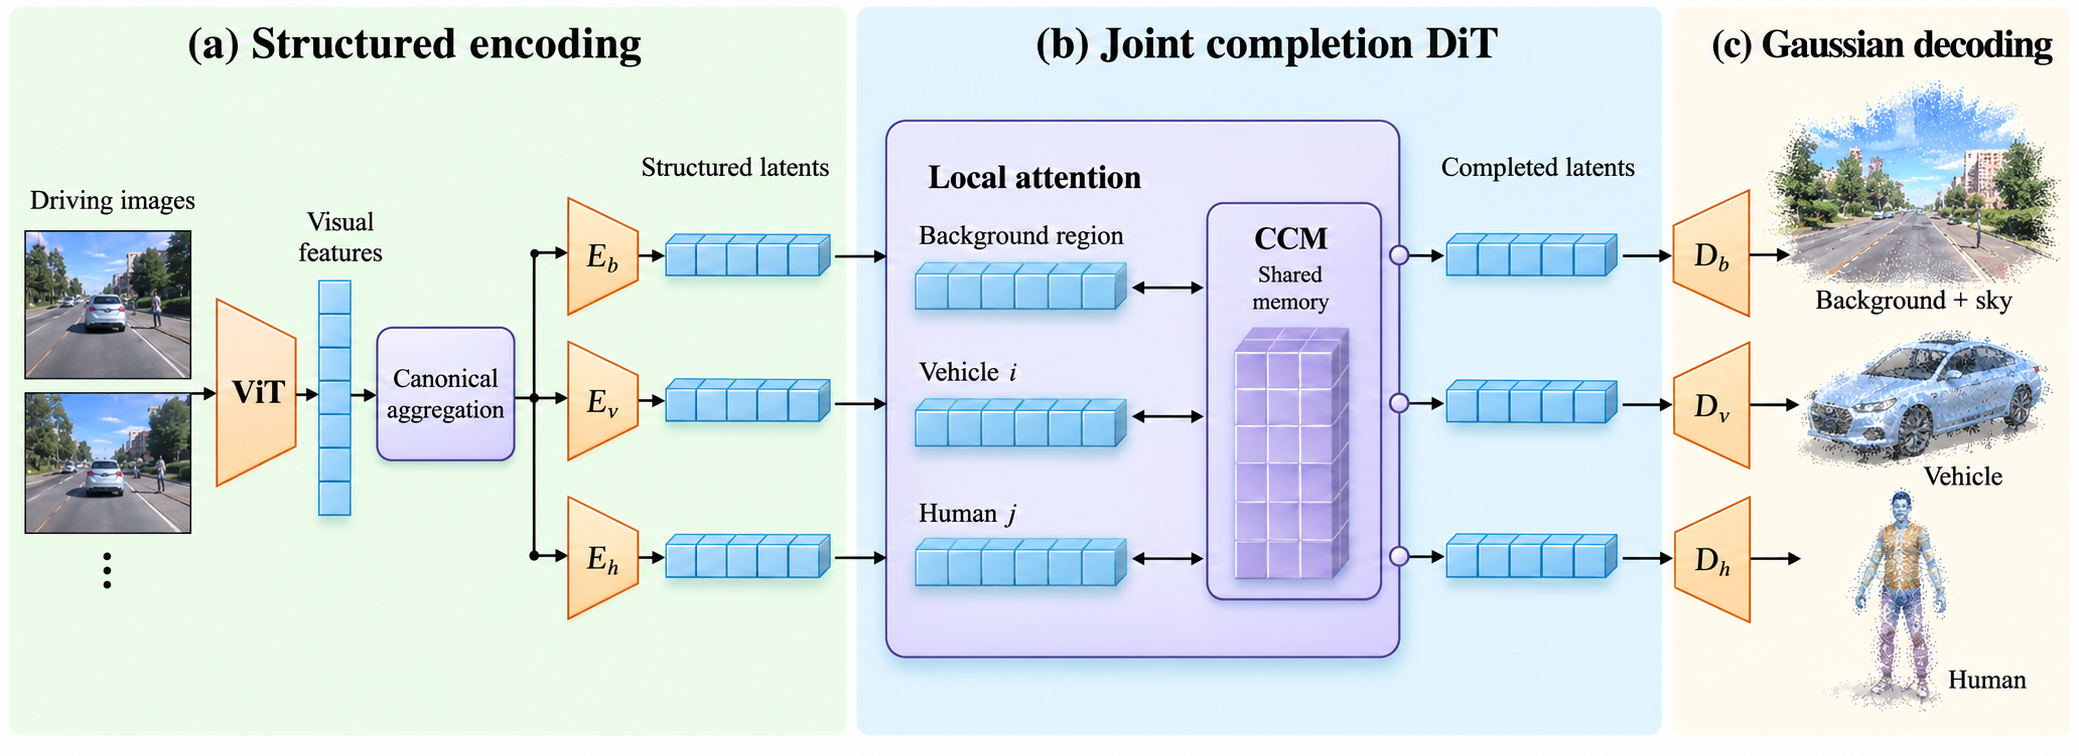
\includegraphics[width=\textwidth]{fig/drivecompose-inference-overview.png}
  \caption{\textbf{DriveCompose 总览。}视觉编码与规范聚合恢复组件特征，类型专属编码器映射结构化潜码，联合补全和高斯解码生成背景、车辆与人体，用于状态驱动组合。场景与资产画面均为机制示意。}
  \label{fig:overview}
\end{figure*}

\subsection{问题定义与可组合表示}
\label{sec:representation}

输入是同步图像日志 $\mathbf I_{t,v}$、时间戳、相机内参及相机到传感器支架的标定。受控评价给定支架位姿、实例身份、车辆框与根轨迹，以及目标人体关节。人体体型与绑定由上下文恢复，重建不使用目标 RGB 或测试 LiDAR。坐标约定与图像预处理见补充材料附录 D。

输出为可组合高斯场景

\begin{equation}
\mathcal W=\bigl(\mathcal G_b,C_{\rm sky},V_{\rm sky},
\{\mathcal A_a\},\mathcal B,\xi\bigr),
\label{eq:world}
\end{equation}

其中，$\mathcal G_b$ 是世界空间背景，$C_{\rm sky}$ 是天空立方体贴图，$V_{\rm sky}$ 表示其有效方向，$\mathcal A_a$ 是身份 $a$ 对应的规范资产，$\mathcal B$ 是有限空间支撑，$\xi$ 是采样种子。这些组件通过高斯泼溅渲染~\cite{kerbl2023gaussians}。车辆表示为局部几何与尺寸固定的刚体资产，人体另存静止骨架和蒙皮权重。场景状态控制这些固定组件的放置与关节运动。

我们通过条件生成建模缺失内容。令 $\mathcal Q$ 为恢复得到的查询布局，$C$ 为其观测证据。补全模型采样未知潜码 $\mathbf z_u$，编解码器 $D_\psi$ 将组合后的潜码解码为场景内容：

\begin{equation}
\mathbf z_u\sim p_\theta(\mathbf z_u\mid C,\mathcal Q),
\qquad
\mathcal W=D_\psi(\mathbf z^{\rm obs},\mathbf z_u;\mathcal Q).
\label{eq:generative-reconstruction}
\end{equation}

查询布局为每个潜码指定空间位置和所属组件。补全在这一布局中生成未知潜码，解码后仍保留其组件身份与运动绑定。

\subsection{视觉恢复与规范聚合}
\label{sec:visual-encoding}

Driving Log Encoder 从各图像提取 patch 特征，并在相机与时间戳之间交换池化上下文~\cite{dosovitskiy2021vit,vaswani2017attention}。几何预测头输出相机光轴深度、法线、置信度、语义和实例归属，将图像特征关联到三维表面及其所属组件。轨迹级身份槽将持久身份、尺寸和人体体型与逐帧变化的根位姿、关节旋转分开表示。网络结构与状态参数化细节见补充材料附录 D。

\label{sec:queries}

\paragraph{空间支撑。}

每个查询存储规范位置 $\mathbf q_i$、单元尺度 $\boldsymbol\delta_i$、类型 $k_i$、局部注意力组 $g_i$ 和参考世界坐标 $\mathbf q_i^w$。可靠深度样本提供表面锚点。背景锚点与有限世界网格结合；刚体锚点经逆 SE(3) 变换对齐后，与局部包围体中的网格结合。人体查询位于规范模板表面，天空查询为按立方体贴图面分组的单位方向。这些支撑为已见与缺失内容提供明确位置。

固定布局以规范坐标标识组件内容，以第一帧世界坐标 $\mathbf q_i^w$（包括人体蒙皮）联系组件与周围场景。

\paragraph{运动感知证据聚合。}

对于每份观测，我们将规范查询放到对应的资产状态：

\begin{equation}
\mathbf p_i(t)=
\begin{cases}
\mathbf q_i,& k_i=\mathrm{background},\\
\operatorname{xyz}(\mathbf T^w_a(t)\bar{\mathbf q}_i),& k_i=\mathrm{rigid},\\
\operatorname{xyz}(\mathbf T^w_h(t)\mathbf A_i(t)\bar{\mathbf q}_i),& k_i=\mathrm{human}.
\end{cases}
\label{eq:query-placement}
\end{equation}

其中，$\bar{\mathbf q}_i$ 为齐次坐标，$\operatorname{xyz}$ 提取欧氏坐标，$\mathbf A_i(t)$ 为加权蒙皮变换。投影得到查询深度 $z_{i,t,v}$，并采样图像特征 $\boldsymbol\phi_{i,t,v}$、深度 $d_{i,t,v}$ 和置信度 $c_{i,t,v}$，按置信度及归一化深度残差 $r=(d-z)/(\eta_{\rm abs}+\eta_{\rm rel}d)$ 为观测赋权。指示量 $a_{i,t,v}$ 选择同一实例中可见且深度一致的观测（附录 D）：

\begin{align}
w_{i,t,v}&=a_{i,t,v}c_{i,t,v}\exp(-r_{i,t,v}^2/2),\\
\mathbf h_i&=\frac{\sum_{t,v}w_{i,t,v}[\boldsymbol\phi_{i,t,v};r_{i,t,v}]}
{\max(\varepsilon,\sum_{t,v}w_{i,t,v})}.
\label{eq:aggregation}
\end{align}

掩码 $m_i$、$f_i$ 和 $u_i$ 区分已见表面、射线标记的自由空间和未知内容，满足 $m_i+f_i+u_i=1$。置信度取有效观测的最大值，两份可靠深度射线票确定自由空间标签。天空特征依据相机旋转和天空语义，按观察方向聚合。判定式与投影足迹掩码审计见附录 D。

\subsection{潜表示编码}
\label{sec:codec}

类型专属编码器将 129 维聚合特征及空间支撑 $[\mathbf h_i;\mathbf q_i;\boldsymbol\delta_i]$ 输入带 LayerNorm 的 $135\!\rightarrow\!128\!\rightarrow\!128$ MLP，得到 $D=128$ 维潜码，并保留查询类型、归属和坐标系。部分与完整分支共享此映射，掩码和置信度单独作为补全条件。未观测潜码置零，已见码记为 $\mathbf z^{\rm obs}$。

\subsection{联合潜空间补全}
\label{sec:completion}

\begin{figure}[t]
  \centering
  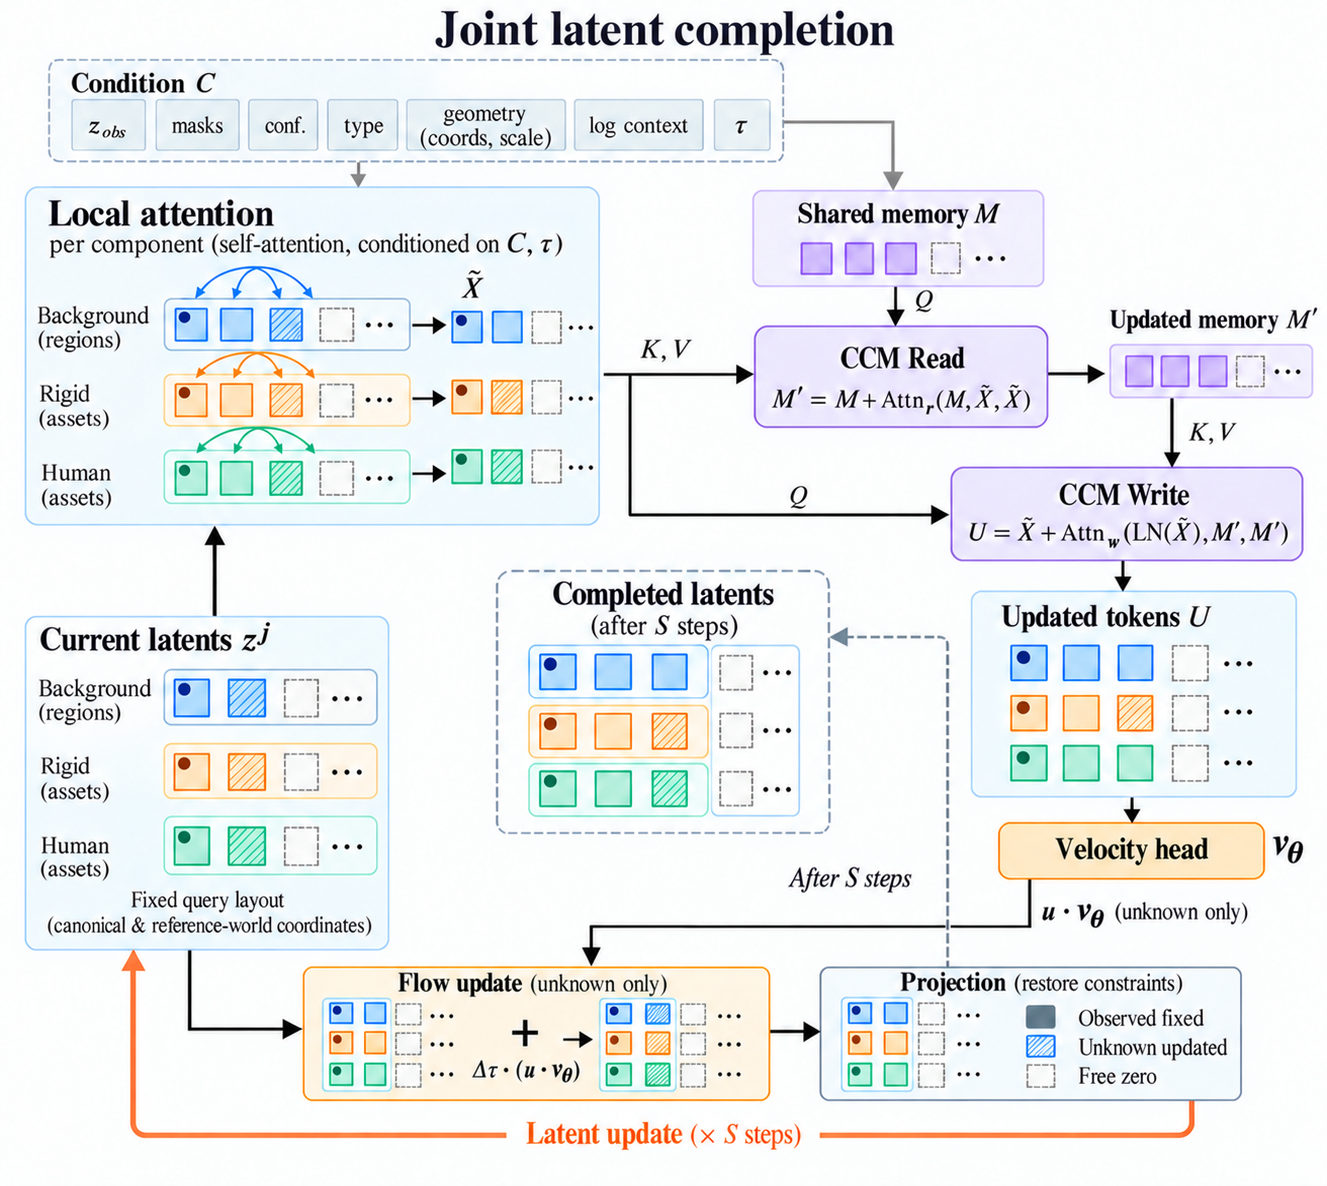
\includegraphics[width=\linewidth]{fig/drivecompose-joint-completion.png}
  \caption{\textbf{联合潜空间补全。}CCM 读入局部特征并回写共享上下文，投影约束流更新只改变未知码。附录 L 提供放大图。}
  \label{fig:joint-completion}
\end{figure}

\paragraph{生成式补全模块。}

生成式补全模块（Generative Completion Module，GCM）由场景条件流 Transformer 与约束采样组成（图~\ref{fig:joint-completion}）。我们采用 DiT 风格的 Transformer~\cite{peebles2023dit} 参数化补全速度场，并通过流匹配训练~\cite{lipman2022flowmatching}。输入结合当前潜码、已见潜码、掩码、置信度、类型、两种坐标描述、单元尺度和池化日志特征。背景按空间邻域分组，每个资产构成一个局部组，天空方向按立方体贴图面分组。局部自注意力分别处理各组，跨组件记忆模块（Cross-Component Memory，CCM）随后通过共享记忆交换上下文：

\begin{align}
\mathbf M'&=\mathbf M+\operatorname{Attn}_{r}
(\mathbf M,\widetilde{\mathbf X},\widetilde{\mathbf X}),\\
\mathbf U&=\widetilde{\mathbf X}+\operatorname{Attn}_{w}
(\operatorname{LN}(\widetilde{\mathbf X}),\mathbf M',\mathbf M').
\label{eq:memory-exchange}
\end{align}

其中，$\widetilde{\mathbf X}$ 拼接局部 token，注意力参数依次为查询、键和值。$\mathbf U$ 后接残差前馈更新。流时间调制局部归一化，记忆由可学习 token 与日志摘要初始化。

\paragraph{流训练与约束采样。}

令 $\mathbf z_1$ 为同一查询布局上的完整目标，$\boldsymbol\epsilon\sim\mathcal N(0,\mathbf I)$ 为高斯噪声。在流时间 $\tau\in[0,1]$，我们仅对未知内容插值：

\begin{equation}
\mathbf z_\tau=m\odot\mathbf z^{\rm obs}
+u\odot[(1-\tau)\boldsymbol\epsilon+\tau\mathbf z_1].
\label{eq:flow-path}
\end{equation}

已见潜码固定，自由空间潜码保持为零。未知查询的目标速度为 $\mathbf z_1-\boldsymbol\epsilon$。引入可选损失选择器 $s_i$，目标为

\begin{equation}
\mathcal L_{\rm flow}=
\frac{\sum_i u_i s_i\|\mathbf v_\theta(\mathbf z_\tau,\tau,C)_i
-(\mathbf z_{1,i}-\boldsymbol\epsilon_i)\|_2^2}
{D\max(1,\sum_i u_i s_i)}.
\label{eq:flow-loss}
\end{equation}

先验学习使用全部未知查询均具有有效目标的样本，$s_i$ 在这些目标中选择损失项（第~\ref{sec:training} 节）。

推理时，以噪声初始化未知潜码，并执行 $S$ 次 Euler 步，步长为 $\Delta\tau=1/S$：

\begin{equation}
\mathbf z^{j+1}=\Pi_{m,f}\!\left[
\mathbf z^j+\Delta\tau\,u\odot
\mathbf v_\theta(\mathbf z^j,j/S,C)\right].
\label{eq:sampling}
\end{equation}

每步后 $\Pi_{m,f}$ 恢复已见潜码、清零自由空间潜码。种子确定一次补全，解码一次后跨状态复用。

\subsection{分类型高斯解码}
\label{sec:decoding}

背景、刚体和人体高斯解码器分别将每个查询独立映射为中心位于其支撑单元内的 $K=4$ 个子高斯。人体子高斯继承查询的蒙皮权重；刚体子高斯共用所属资产的刚体变换。不透明度乘以 $1-f_i$，使自由空间查询不能产生可见高斯。独立天空头在观测支持的方向域 $V_{\rm sky}$ 内预测立方体贴图颜色。高斯与外观参数化详见补充材料附录 E。

各查询独立解码。冻结编解码器并保留已见潜码，使已见高斯参数保持不变。自由射线损失约束新增高斯对可见性与透明度混合的影响，第~\ref{sec:observation-preservation} 节给出实测。

\subsection{场景组合}
\label{sec:composition}

\paragraph{状态驱动渲染。}

时刻 $k$ 的状态 $s_k$ 指定自车位姿、活动资产、刚体变换，以及人体根位姿与关节姿态。刚体位姿对规范高斯的中心和协方差施加刚体变换，人体关节姿态通过存储的蒙皮权重使高斯变形，补全表面因此随相应身体部位运动。具体变换见补充材料附录 C。渲染器合成背景、活动资产和有效天空：

\begin{equation}
o_k=\mathcal R(\operatorname{Compose}(\mathcal W,s_k),\mathcal C_k).
\label{eq:simulation}
\end{equation}

背景与规范资产保持固定，新相机及参与者状态复用同一份完成内容。

\subsection{训练流程}
\label{sec:training}
训练依次进行视觉恢复、潜表示拟合、补全先验学习和通过渲染适配。部分输入固定 $\mathcal Q$，包括单元尺度、组件归属及人体绑定。完整网格提供各单元内的表面样本，多视图渲染与冻结视觉编码器得到 $\mathbf h_i^{\rm full}$，再由共享的类型专属编码器映射为 $\mathbf z_{1,i}=E_{k_i}([\mathbf h_i^{\rm full};\mathbf q_i;\boldsymbol\delta_i])$。无表面单元采用零特征和不透明度监督。

潜表示拟合结束后，恢复模块和 codec 保持冻结。阶段三使用每个未知查询均具有完整目标的合成样本；阶段四仅更新 GCM，以 $1{:}3$ 混合完整合成样本和 740 条真实训练日志。四阶段共更新 287,360 步，目标构造、网络规模和训练设置详见附录 B。

% 按用户要求逐字保留原压缩包中的实验章节。
\section{实验}
\label{sec:experiments}

\FloatBarrier
\Needspace{13\baselineskip}
\section{讨论}
\label{sec:discussion}

DriveCompose 覆盖有限区域并采用固定照明。观测锚点会继承深度、身份和规范姿态的恢复误差。车辆保持刚体结构；人体使用固定衣物体积与骨架绑定，超出模板支撑的姿态可能暴露缺失内容。参考世界坐标描述构建时的场景，资产移动后的接触与碰撞有效性由物理后端处理。原视角检查约束补全结果与已记录证据的一致性；观测之外的几何以及新状态下的表现仍需分别评估。

\Needspace{14\baselineskip}
\section{结论}
\label{sec:conclusion}

本文提出 DriveCompose，用于可组合驾驶场景的生成式重建。结构化潜表示将图像证据汇入背景与规范资产，使缺失内容在生成之前就具有明确的位置、身份和运动模型。条件补全利用场景上下文并保留已观测证据，类型解码输出可复用高斯场景的组成部分。内容构建与状态驱动装配相分离，使后续相机和资产状态变化能够使用同一次补全结果。

\FloatBarrier
{\small
\bibliographystyle{ieeenat_fullname}
\bibliography{main}
}
\end{document}
